\section{N\'umeros Reais, Fun\c c\~oes e Introdu\c c\~ao a Limites}
\subsection{Exerc\'icios de Fun\c c\~oes e Panorama Geral}
\subsubsection{Exerc\'icio 1}  
\paragraph{}Parte 1 - Se considerarmos 
$$
f(x) = \frac{x^3 + x^2 - x - 1}{x-1}, x\neq{1},
$$
ent\~ao a que classe de fun\c c\~oes ela pertence? Note que se efetuarmos a divis\~ao polinomial, concluiremos que 
$$
\frac{x^3 + x^2 - x - 1}{x-1} = x^2 + 2x + 1.
$$
Isto significa que f \'e uma fun\c c\~ao polinomial de grau 2? Justifique e fa\c ca o passo-a-passo.
\begin{proof*}
	Considere a fun\c c\~ao 
	$$
	f(x) = \frac{x^3 + x^2 - x - 1}{x-1}, x\neq{1},
	$$
	e $p(x) = x^3 + x^2 - x - 1, q(x) = x - 1,$ em que $p:\mathbb{R}\rightarrow\mathbb{R}$ e $q(x)\mathbb{R}/\{1\}\rightarrow\mathbb{R}$ s\~ao polin\^omios. Segue que:
	$$
	f(x) = \frac{x^3 + x^2 - x - 1}{x-1} = \frac{p(x)}{q(x)}, x\neq{1}.
	$$
	Por defini\c c\~ao, uma fun\c c\~ao na forma de quociente de polin\^omios, em que o denominador \'e um polin\^omio com o dom\'inio tal que ele nunca \'e nulo, \'e conhecida como uma fun\c c\~ao racional. 

	No entanto, \'e melhor lidar com fra\c c\~oes de polin\^omios simplificados, ou seja, \'e preciso encontrar o fator comum entre ambos. Observe que, em x = 1, 
	$$
	p(x) = 1^3 + 1^2 - 1 - 1 = 1 + 1 - 1 - 1 = 0
	$$ 
	e 
	$$
	q(x) = 1 - 1 = 0,
	$$ 
	ent\~ao (x-1) \'e um fator comum entre ambos, isto \'e, ele pode ser fatorado ap\'os manipular o polin\^omio p(x) . Assim, note que, somando e subtraindo fatores para que possamos fatorar (x-1) de p(x), chegamos em: 
	$$
	p(x) = x^3 + x^2 - x - 1 = x^3 + (2x^2 - x^2) +(x - 2x) -1 = (x-1)(x^2 + 2x^2 + 1) = q(x)(x^2 + 2x^2 + 1),
	$$
	de forma que:
	$$
	f(x) = \frac{x^3 + x^2 - x - 1}{x-1} = \frac{p(x)}{q(x)} = \frac{q(x)(x^2 + 2x^2 + 1)}{q(x)} = x^2 + 2x^2 + 1, x\neq{1}.
	$$
	Logo, ap\'os efetivada a divis\~ao, obtemos que f \'e uma fun\c c\~ao polinomial de grau 2. 
\qedsymbol
\end{proof*}

\newpage

\paragraph{}Parte 2 - Verifique as seguintes identidades:
\begin{figure}[h!]
	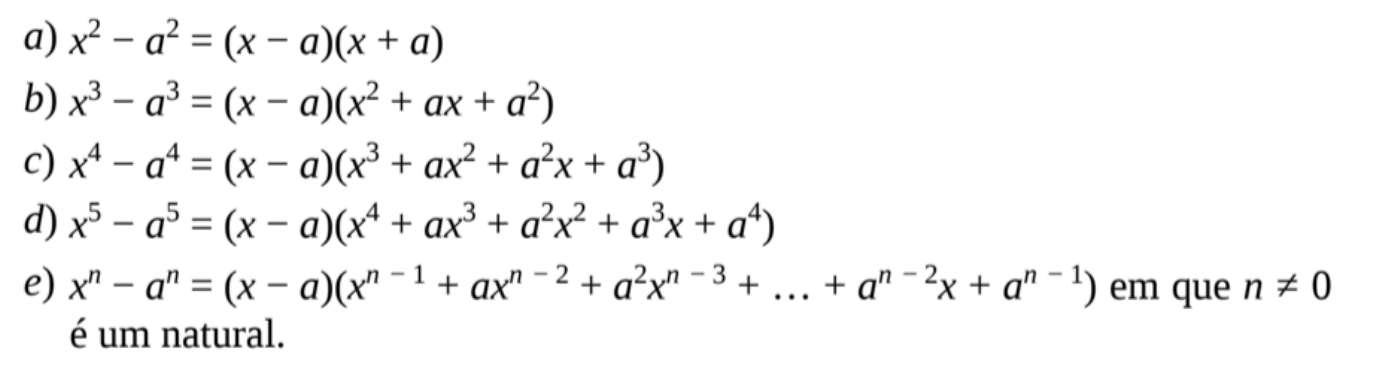
\includegraphics[width=15cm, height=4cm]{identidades.png}
\end{figure}

\begin{proof*}
	Antes da formaliza\c c\~ao da prova, um bom come\c co \'e analisar a imagem cuidadosamente. De fato, ao fazer isso, observe a repeti\c c\~ao do termo (x - a) \`a direita de cada igualdade. Outro ponto not\'avel \'e que, para cada n, ocorre uma expans\~ao de $\sum_{i=0}^{n}a^ix^{n-i-1}$ ao lado de (x - a), em que $n\in\mathbb{N}$. Em outras palavras, isso est\'a indicando fortemente a presen\c ca de uma hip\'otese indutiva para demonstrar o resultado. 
	
	Com  efeito, provemos o caso base do item a, ou seja, n = 2. Considere o produto (x-a)(x+a):
	$$
	(x - a)(x + a) = x^2 + xa - ax - a^2 = x^2 + ax - ax - a^2 = x^2 - a ^2.
	$$
	Destarte, obtivemos o caso base como verdadeiro. Nessa linha de racioc\'inio, a hip\'otese indutiva afirma que, dado uma base verdadeira, o resultado ser\'a provado se, assumindo o caso n-1 como verdade, o caso n tamb\'em ser\'a (pois assim, o caso 1 sendo verdadeiro implica que o 2 tamb\'em \'e, consequentemente o 3, o 4, etc.). Suponha que o resultado vale para n - 1, isto \'e, para $n\neq{0}$ 
	$$	
	x^{n - 1} - a^{n - 1} = (x - a)\biggl(\sum_{i=0}^{n-2}a^ix^{n-i-2}\biggr).
	$$
	Em part\'icular, somando $2a^{n-1}, $segue que:
	$$
	x^{n - 1} + a^{n - 1} = (x - a)\biggl(\sum_{i=0}^{n-2}a^ix^{n-i-2}\biggr) + 2a^{n-1}.
	$$
	Multiplicando ambos os lados por (x-a), chegamos em:
	$$
	(x - a)\biggl(\sum_{i=0}^{n-1}a^ix^{n-i-1}\biggr)  = (x - a)(x^{n-1} + \biggl(\sum_{i=1}^{n-2}a^ix^{n-i-1}\biggr) + a^{n-1})  = (x - a)(x^{n-1} + a^{n-1} + \biggl(\sum_{i=1}^{n-2}a^ix^{n-i-1}\biggr))  = 
	$$
	$$
	= (x - a)(2a^{n-1} + (x - a)\biggl(\sum_{i=0}^{n-2}a^ix^{n-i-2}\biggr) + \biggl(\sum_{i=1}^{n-2}a^ix^{n-i-1}\biggr))  = (x - a)(2a^{n-1} + x^{n-1} - a^{n-1} + \biggl(\sum_{i=1}^{n-2}a^ix^{n-i-1}\biggr)) = 
	$$
	$$
	= 2xa^{n-1} - 2a^n + (x-a)\biggl(x^{n-1} - a^{n-1} + \biggl(\sum_{i=1}^{n-2}a^ix^{n-i-1}\biggr)\biggr) = 2xa^{n-1} - 2a^n + x^{n} - xa^{n-1} -a^{n-1}x + a^{n} + (x-a)\biggl(\sum_{i=1}^{n-2}a^ix^{n-i-1}\biggr)\biggr) = 
	$$
	$$
	= xa^{n-1} - a^n + x^{n} - xa^{n-1} + (x-a)\sum_{i=1}^{n-2}a^ix^{n-i-1} = (x^n - a^n) + (xa^{n-1} - ax^{n-1} + (x-a)\sum_{i=1}^{n-2}a^ix^{n-i-1}) .
	$$
Analisemos o termo $(x-a)\sum_{i=1}^{n-2}a^ix^{n-i-1}$ antes de prosseguir. Temos:
	$$
	(x-a)\sum_{i=1}^{n-2}a^ix^{n-i-1} = x\sum_{i=1}^{n-2}a^ix^{n-i-1} - a\sum_{i=1}^{n-2}a^ix^{n-i-1} = \sum_{i=1}^{n-2}a^ix^{n-i} - \sum_{i=1}^{n-2}a^{i+1}x^{n-i-1} = 
	$$
	$$
	= ax^{n-1} + a^2x^{n-2} + \cdots + a^{n-2}x^2 - a^2x^{n-2} - ... -a^{n-2}x^2 - a^{n-1}x = ax^{n-1} - a^{n-1}x.
	$$
Juntando isso com a conta anterior, chegamos, finalmente, em:
	$$
	(x^n - a^n) + (xa^{n-1} - ax^{n-1} + (x-a)\sum_{i=1}^{n-2}a^ix^{n-i-1}) = (x^n - a^n) + (xa^{n-1} - ax^{n-1} + ax^{n-1} - a^{n-1}x ) =
	$$
	$$
	= x^n - a^n + 0 = x^n - a^n.
	$$
Portanto, 
	$$
	(x - a)\biggl(\sum_{i=0}^{n-1}a^ix^{n-i-1}\biggr) = x^n - a^n.
	$$
Agora que provamos isso, utilizando n = 3, 4, 5, mostramos as identidades que faltam:
\begin{itemize}
\item[n=3:] $$ x^3 - a^3 = (x-a)\sum_{i=0}^{2}a^ix^{2-i} = (x-a)(a^2 + ax + x^2). $$
\item[n=4:] $$ x^4 - a^4 = (x-a)\sum_{i=0}^{3}a^ix^{3-i} = (x-a)(a^3 + a^2x + ax^2 + x^3). $$
\item[n=5:] $$ x^5 - a^5 = (x-a)\sum_{i=0}^{4}a^ix^{4-i} = (x-a)(a^4 + a^3x + a^2x^2 + ax^3 + x^4).$$
\end{itemize}
\qedsymbol	
\end{proof*}

\subsubsection{Exerc\'icio 2} 
\paragraph{}Parte 1 - Fazendo todos os detalhes e explicando todos os passos, explicite o dom\'inio de cada umas das fun\c c\~oes abaixo e calcule os produtos $f\cdot{}g, g\cdot{}h \text{ e } h\cdot{}i$, em que:
$$
f(x) = 2x^3 - 5x^2 + 3, \hspace{0.5cm}
g(x) = 3x^2 - x + 2, \hspace{0.5cm}
h(x) = \frac{x^2 - 1}{x - 3} \hspace{0.2cm} \text{\&} \hspace{0.2cm}   
i(x) = \frac{x^3 - 1}{x^2 + 1}
$$
\begin{sol*}
A priori, analisemos os dom\'inios de cada uma das fun\c c\~oes. Come\c cando por f, levando em conta que, quando n\~ao explicitado, o dom\'inio de uma fun\c c\~ao \'e o maior subconjunto de $\mathbb{R}$ em que faz sentido defin\'i-la, temos $D_f = \mathbb{R}$, pois a fun\c c\~ao n\~ao possui pontos problem\'aticos (com isso, queremos dizer um ponto em que, por exemplo, ter\'iamos $\frac{1}{0}$ ou $\sqrt{-x}, x > 0$ e $x\in\mathbb{R}.$) Analogamente, segue que o dom\'inio de g tamb\'em \'e $D_g = \mathbb{R}.$ 

Contudo, ao lidarmos com os dom\'inios de h e i, \'e necess\'ario ter cautela, j\'a que s\~ao definidas por fra\c c\~oes. No caso de h, seu dom\'inio \'e o conjunto dos reais tais que x - 3 n\~ao \'e nulo, ou seja, 
$$
D_h = \{x\in\mathbb{R}: x - 3 \neq 0\} = \mathbb{R}/\{3\}.
$$
Em primeira vista, o caso da fun\c c\~ao i pode parecer o mesmo, ou seja, que vai ser definido como o conjunto dos reais a menos de um conjunto finito de pontos. No entanto, note que, para isso, seria preciso que $x^2 + 1 = 0, x\in\mathbb{R},$ o que nunca acontece (nos reais!). Portanto, i est\'a definido em $D_{i} = \mathbb{R}$.

Ademais, a forma de realizar produtos entre fun\c c\~oes deve ser esclarecida: O produto entre duas fun\c c\~oes f e g, definido ponto-a-ponto, \'e dado por
$$
(f\cdot{g})(x) = f(x) \cdot{g(x)}.
$$
Com isso em mente, vamos aos c\'alculos:
\begin{itemize}
\item[i.)] $f\cdot{g}$ (produto de f com g)
$$
(f \cdot{g})(x) = f(x)\cdot{g(x)} = (2x^3 - 5x^2 + 3)\cdot(3x^2 - x + 2) = 2x^3(3x^2 - x + 2) - 5x^2 (3x^2 - x + 2) + 3(3x^2 - x + 2) = 
$$
$$
= 6x^5 - 2x^4 + 4x^3 - 15x^4 + 5x^3 - 10x^2 + 9x^2 - 3x + 6 = 6x^5 - 17x^4 + 9x^3 - x^2 + 6
$$
\item[ii.)]$g\cdot{h}$  (produto de g com h)
$$
(g\cdot{h})(x) = g(x)\cdot{h(x)} = (3x^2 - x + 2)\cdot\biggl(\frac{x^2 - 1}{x - 3}\biggr) = \biggl(\frac{(3x^2 - x + 2)(x^2 - 1)}{x - 3}\biggr) = 
$$
$$
= \biggl(\frac{3x^4 - 3x^2 - x^3 + x + 2x^2 - 2}{x - 3}\biggr) = \biggl(\frac{3x^4 - x^2 - x^3 + x - 2}{x - 3}\biggr)
$$
\item[iii.)]$h\cdot{i}$ (produto de h com i)
$$
(h\cdot{i})(x) = h(x)\cdot{i(x)} = \biggl(\frac{x^2 - 1}{x - 3}\biggr)\biggl(\frac{x^3 - 1}{x^2 + 1}\biggr) = \biggl(\frac{(x^2 - 1)(x^3 - 1)}{(x - 3)(x^2 + 1)}\biggr) 
$$
$$
= \biggl(\frac{x^5 - x^2 -x^3 + 1}{x^3 + x - 3x^2 - 3}\biggr) 
$$
\end{itemize}
\qedsymbol
\end{sol*}

\paragraph{}Parte 2 - Sabendo que $\sin{x}$ n\~ao \'e uma fun\c c\~ao racional, mostre que a fun\c c\~ao $\tan{x}$ n\~ao pode ser uma fun\c c\~ao racional.
\begin{proof*}
A priori, sabemos que, para uma fun\c c\~ao ser racional, ela deve ser o quociente de dois polin\^omios. Analogamente, se uma fun\c c\~ao n\~ao \'e racional, ela n\~ao pode ser escrita como o quociente de dois polin\^omios. 

A posteriori, suponha que $\sin{x}$ n\~ao \'e uma fun\c c\~ao racional. Defina 
$$
\tan(x) = \frac{\sin(x)}{\cos(x)}.
$$
Desta forma, segue de cara que $\tan(x)$ n\~ao \'e uma fun\c c\~ao racional, pois um de seus componentes, no caso, $\sin(x)$, n\~ao pode ser escrito como o quociente de dois polin\^omios, de forma que, mesmo se $\cos(x)$ fosse racional, ainda assim seria imposs\'ivel escrev\^e-la como o quociente desejado. Portanto, a tangente $\tan(x)$ n\~ao pode ser uma fun\c c\~ao racional.
\qedsymbol
\end{proof*}

\subsubsection{Exerc\'icio 3}
\paragraph{}Parte 1  - Defina os conceitos de injetividade e sobrejetividade.
\begin{sol*}
Antes de defin\'i-los explicitamente, \'e importante conhecer um pouco de suas utilidades. O primeiro deles, a injetividade, lida com a quest\~ao da unicidade na imagem da fun\c c\~ao, tanto \'e que tamb\'em \'e conhecido como fun\c c\~ao 1-1, enquanto a sobrejetividade lida com o ``alcance'' da fun\c c\~ao. Se ambos os casos ocorrem, chamamos a fun\c c\~ao de bije\c c\~ao, uma classe muito importante pois ela relaciona cada elemento de cada um dos conjuntos (o dom\'inio e o contra-dom\'inio) unicamente, de forma que h\'a um inverso pra fun\c c\~ao, mas isso \'e outro t\'opico. 

Destarte, definamos ambas matematicamente. Dados dois conjuntos A e B n\~ao-vazios, seja $f:A\rightarrow{B}$ uma fun\c c\~ao entre os dois conjuntos. Dizemos que:
\begin{itemize}
\item[a)] f \'e uma fun\c c\~ao injetora se, para $a_1, a_2\in{A}, f(a_1) = f(a_2)$ implica que $a_1 =  a_2.$
\item[b)] f \'e uma fun\c c\~ao sobrejetora se, dado $b\in{B}$, existe (pelo menos) um elemento $a\in{A}$ tal que $f(a) = b.$
\end{itemize}

Com essas defini\c c\~oes em mente, retomemos o primeiro par\'agrafo. A unicidade mencionada segue pois, para uma aplica\c c\~ao qualquer de A em B ser uma fun\c c\~ao, ela precisa que, dados $a_1, a_2\in{A}$, caso $a_1 = a_2, f(a_1) = f(a_2)$. A injetividade diz o oposto, ou seja, se $f(a_1) = f(a_2), a_1 = a_2$. Juntando os dois, uma fun\c c~ao injetora obedece $f(a_1) = f(a_2) \text{ se, e somente se, } a_1 = a_2,$ dados $a_1, a_2\in{A},$ tal que cada elemento de um conjunto define unicamente um elemento no outro. Quanto \`a sobrejetividade, ela define quando uma fun\c c\~ao tem alcance m\'aximo, pois como cada $b\in{B}$ pode ser escrito como a fun\c c\~ao aplicada a algum elemento de A, segue que $B \subset f(A)$, tal que, como por defini\c c\~ao $f(A) \subset B$, temos $f(A) = B$, ou seja, a imagem da fun\c c\~ao \'e o contra-dom\'inio inteiro.
\qedsymbol
\end{sol*}

\paragraph{}Parte 2 - Mostre que a fun\c c\~ao $f(x) = \sin(x), x\in[0, \pi]$ n\~ao \'e injetora, mas para $x\in[0, \frac{\pi}{2}]$ ela \'e.
\begin{proof*}
Vamos mostrar uma contradi\c c\~ao engra\c cada. Suponha que, de fato, $f(x) = \sin(x)$ \'e injetora no intervalo $[0, \pi]$. Em particular, temos:
$$
\sin(0) = 0 = \sin(\pi) \Rightarrow 0 = \pi.
$$
Se isso fosse verdade, alguns desastres aconteceriam. Dentre eles, n\~ao existiriam c\'irculos, pois todos eles poderiam ser vistos como pontos, j\'a que sua \'area, $\pi\cdot{r^2} = 0$ para todo r, ou seja, tamb\'em n\~ao existiria engenharia e, quem sabe, nem mesmo o universo. Isso est\'a obviamente errado. Logo, $\sin(x)$ n\~ao pode ser injetora em $[0, \pi].$ 

De lado com os cataclismas e fins do mundo, considere, agora, o intervalo $[0, \frac{\pi}{2}].$ Sabemos que a fun\c c\~ao seno \'e estritamente crescente nesse intervalo, que \'e o primeiro quadrante. Assim, temos, para $x, y\in[0, \frac{\pi}{2}],$
$$
\sin(x) < \sin(y), x < y \text{ ou } \sin(x) > \sin(y), x > y.
$$
Assim, a \'unica forma de $\sin(x) = \sin(y)$ \'e quando x = y, que \'e a exata defini\c c\~ao de uma fun\c c\~ao injetora.
\qedsymbol
\end{proof*}

\paragraph{}Parte 3 - Fa\c ca as seguintes composi\c c\~oes: $f\circ{g}, g\circ{f}, f\circ{h} \text{ e } h\circ{f}$, em que:
$$
f(x) = -3x + 2, \hspace{0.5cm} g(x) = 3x^2 - x  + 2, \hspace{0.2cm} \text{ e } \hspace{0.2cm} h(x) = \frac{x^2 - 1}{x - 3}.
$$
\begin{sol*}
Antes de dar in\'icio \`as contas propriamente ditas, note que, ao compor h com f, ou f com h, o dom\'inio de f mudar\'a de $D_f = \mathbb{R}$ para $D_f = \mathbb{R}/\{3\}.$ Feita essa observa\c c\~ao, sigamos em frente:
\begin{itemize}
\item[i)]$$(f\circ{g})(x) = f(g(x)) = f(3x^2 - x + 2) = -3(3x^2 - x + 2) + 2 = -9x^2 + 3x - 6 + 2 = -9x^2 + 3x - 4.$$
\item[ii)]$(g\circ{f})(x)$
$$
(g\circ{f})(x) = g(f(x)) = g(-3x + 2) = 3(-3x + 2)^2 +3x - 2 + 2 =
$$
$$
= 3(9x^2 - 12x + 4) + 3x = 27x^2 - 36x + 12 + 3x = 27x^2 - 33x + 12.
$$
\item[iii)]$(f\circ{h})(x)$
$$
(f\circ{h})(x) = f(h(x)) = f(\frac{x^2 - 1}{x - 3}) = -3\biggl(\frac{x^2 - 1}{x - 3}\biggr) + 2 = 
$$
$$
= \frac{-3x^2 + 3}{x-3} + 2 = \frac{-3x^2 + 3 + 2x - 6}{x-3} = \frac{-3x^2 + 2x -3}{x-3}.
$$
\item[iv)]$(h\circ{f})(x) $
$$
(h\circ{f})(x) = h(f(x)) = h(-3x + 2) = \frac{(-3x + 2)^2 - 1}{-3x+2 - 3} = \frac{9x^2 -12x + 4 - 1}{-3x -1} = -\frac{3(3x^2 - 4x + 1)}{3x+1}
$$
\end{itemize} 
\qedsymbol
\end{sol*}
\subsection{Um Panorama Geral}
\subsubsection{Exerc\'icio 4}
\paragraph{} Parte 1 - Quais s\~ao os dois principais problemas a que se refere o C\'alculo diferencial e integral?
\begin{sol*}
O c\'alculo pode ser visto como o estudo de ``infinitos'', ent\~ao, partindo desse princ\'ipio, \'e poss\'ivel iluminar a mente com rela\c c\~ao \`a resposta para essa pergunta. Nessa linha de racioc\'inio, o c\'alculo diferencial \'e apresentado, normalmente, com o problema de motiva\c c\~ao da reta tangente e do passo de uma fun\c c\~ao. Explicitamente falando, a busca do ponto \'unico para cada reta tangente e o que acontece com a fra\c c\~ao $\frac{\Delta{f(x)}}{\Delta{x}}$ quando $\Delta{x}$ fica cada vez menor, ou seja, como uma mudan\c ca at\'e a vizinhan\c c\a imediata de x afeta sua fun\c c\~ao f(x). Em ess\^encia, ambos os problemas s\~ao os mesmos, pois lidam com a taxa de varia\c c\~ao de x em n\'iveis infinitesimais, da\'i que vem a parte do c\'alculo diferencial que estuda infinitos, mas s\~ao as coisas infinitamente pequenas.

Tratando-se do c\'alculo integral, diferente da busca pela taxa de varia\c c\~ao, ele lida com as \'areas de gr\'aficos de fun\c c\~oes, isto \'e, como calcular a \'area de um gr\'afico arbitr\'ario. Para isso, a no\c c\~ao de infinito como mencionada previamenta aparece em forma de aproxima\c c\~oes cada vez mais finas por meio de ret\^angulos que possuem tamanhos maiores ou menores para uma dada sec\c c\~ao do gr\'afico. Quanto mais ret\^angulos forem usados, ou seja, quando menor forem seus tamanhos, mas maiores forem seus n\'umeros, melhor ser\'a a aproxima\c c\~ao da \'area de dada fun\c c\~ao, tal que, quando alcan\c cados infinitos ret\^angulos, a \'area da figura formada pelo gr\'afico \'e exata. Essa forma\c c\~ao de ret\^angulos cada vez menores tamb\'em pode ser compreendida como uma divis\~ao do intervalo da reta que representa o dom\'inio da fun\c c\~ao em partes iguais cada vez menores, tal que quanto maior o n\'umero de partes, melhor a aproxima\c c\~ao, at\'e que, novamente, com infinitas partes, chega-se no valor exato da \'area da fun\c c\~ao.
\qedsymbol
\end{sol*}

\paragraph{} Parte 2 - Utilize a constru\c c\~ao da secante ao gr\'afico para obter a tangente, em que $f(x) = x^5$, explicitando a reta tangente no ponto (a, f(a)) e deixando claro como obteve o coeficiente angular desta reta.
\begin{sol*}
Antes de tudo, lembre-se que uma reta secante a um gr\'afico \'e tal que ela passa por exatos dois pontos dele. Considerando que o que liga dois pontos \'e uma reta, a secante pode ser interpretada como a taxa de varia\c c\~ao da fun\c c\~ao em dois pontos $x, x_0\in{D_f}$ dados. Em outras palavras, se S for a secante, temos
$$
S = \frac{f(x) - f(x_0)}{x - x_0} = \frac{\Delta{f(x)}}{\Delta{x}}.
$$
Retome, agora, o exer\c c\'icio 4.1. A palavra "taxa de varia\c c\~ao" tamb\'em aparece l\'a, ent\~ao, consequentemente, a secante apareceu. Vamos seguir nessa linha de racioc\'inio, junto com a no\c c\~ao de infinitesimalidade, para obter a taxa de varia\c c\~ao imediata (Nome chique para derivada) de f no ponto $x_0$. Com efeito, a varia\c c\~ao imediata \'e o valor de S quando $x$ se torna $a$ e, para isso, utilizemos a no\c c\~ao de limite:
$$
\lim_{x\to{a}} S = \lim_{x\to{a}}\biggl(\frac{f(x) - f(a)}{x - a}\biggr) = \lim_{x\to{a}}\biggl(\frac{x^5 - a^5}{x - a}\biggr) = \lim_{x\to{a}}\biggl(\sum_{n=0}^{4}a^nx^{4-n}\biggr) = \sum_{n=0}^{4}a^n\lim_{x\to{a}}x^{4-n}= 
$$
$$
= \sum_{n=0}^{4}a^na^{4-n} = \sum_{n=0}^{4}a^{n+4-n} = \sum_{n=0}^{4}a^4 = 5a^4 .
$$
Como esse valor \'e exato e, consequentemente uma reta passando em um ponto s\'o, ele representa a tangente em (a, f(a)) com coeficiente angular igual a 5, pois a soma possui 5 termos, independentes do \'indice, $a^4$ iguais (apesar de n = 4, a soma come\c ca do 0, ent\~ao s\~ao n+1 = 5 termos). Esse processo pode, de fato, ser generalizado para um mon\^omio de grau n, $f(x) = x^n$, para obtermos que a tangente ao ponto $(x_0, f(x_0))$ \'e dada por $nx^{n-1}.$ Essa regra de obten\c c\~ao da tangente de um mon\^omio \'e mais conhecida como regra do tombo em cursos iniciantes, e \'e uma das bases para fazer a maioria das deriva\c c\~oes do C\'alculo diferencial. Uma observa\c c\~ao interessante, para finalizar, \'e o uso do exerc\'icio 1.1 parte 2 para chegar no resultado que quer\'iamos, sendo este o caso em que n = 4 dividido por (x - a).
\qedsymbol
\end{sol*}

\paragraph{} Parte 3 - Calcule a \'area de $f(x) = x^3$ dividindo o intervalo $[0, 1]$ em 7 parte iguais. Qual o valor aproximado da \'area a que se chega? Dividindo-se o intervalo em mais partes, digamos $\lfloor{\pi}\rfloor\cdot{10^{36}}$, espera-se que esta aproxima\c c\~ao do valor real da \'area melhore ou piore?
\begin{sol*}
A priori, dividiremos o intervalo em 7 partes iguais, ou seja, I = [0, 1] se quebra nos seguintes peda\c cos:
$$
I_1 = \biggl[0, \frac{1}{7}\biggr],     I_2 = \biggl[\frac{1}{7}, \frac{2}{7}\biggr],       I_3 = \biggl[\frac{2}{7}, \frac{3}{7}\biggr],    I_4 = \biggl[\frac{3}{7}, \frac{4}{7}\biggr],    I_5 = \biggl[\frac{4}{7}, \frac{5}{7}\biggr], I_6 = \biggl[\frac{5}{7}, \frac{6}{7}\biggr], I_7 = \biggl[\frac{6}{7}, 1\biggr].
$$
Agora, vejamos como a fun\c c\~ao f(x) se comporta neles, ou melhor, como sua \'area \'e influenciada por deslocamentos ao longo de cada peda\c co de I. O princ\'ipio por tr\'as desse processo \'e aproximar \'area por ret\^angulos menores que a total e depois por ret\^angulos maiores que ela. Comecemos, ent\~ao, por esses menores, ou seja, analisemos o valor de f nos pontos da esquerda dos intervalos. Em seguida, somaremos eles, dividindo pelo n\'umero de divis\~oes, no caso, 7, e repetiremos para os pontos \`a direita dos intervalos. Segue que 
$$
L_7 = \frac{1}{7}\biggl(f(0) + f(\frac{1}{7}) + f(\frac{2}{7}) + f(\frac{3}{7}) + f(\frac{4}{7}) + f(\frac{5}{7}) + f(\frac{6}{7})\biggr) =
$$
$$
\frac{1}{7}(0 + \frac{1}{7^3}(1^3 + 2^3 + 3^3 + 4^3 + 5^3 + 6^3)) = \frac{1}{7^4}\biggl(1^3 + 2^3 + 3^3 + 4^3 + 5^3 + 6^3\biggr) = \frac{441}{7^4}
= 0.183.$$
Repetindo o processo para os n\'umeros das pontas direitas dos intervalos, temos:
$$
R_7 = \frac{1}{7}\biggl(f(\frac{1}{7}) + f(\frac{2}{7}) + f(\frac{3}{7}) + f(\frac{4}{7}) + f(\frac{5}{7}) + f(\frac{6}{7}) + f(1)\biggr) =
$$
$$
\frac{1}{7}(\frac{1}{7^3}(1^3 + 2^3 + 3^3 + 4^3 + 5^3 + 6^3) + 1) = \frac{1}{7^4}\biggl(1^3 + 2^3 + 3^3 + 4^3 + 5^3 + 6^3\biggr) + \frac{1}{7} = \frac{441}{7^4} + \frac{1}{7}= 0.183 + 0.142 = 0.325.
$$
Assim, obtemos que a \'area da fun\c c\~ao, A, \'e tal que:
$$
L_7 < A < R_7.
$$
	\par{}Ademais, dividindo-se o intervalo em $3\cdot{10^{36}} = \lfloor{\pi}\rfloor\cdot{10^{36}}$ partes iguais, note que os ret\^angulos se tornam mais numerosos e com bases menores. Assim, a \'area individual de cada um deles ser\'a menor, tal que, ao som\'a-los, chegaremos em uma \'area mais aproximada, uma aproxima\c c\~ao mais refinada do valor da \'area da fun\c c\~ao. Isso esconde o principal mecanismo da soma de Riemann, ou seja, da defini\c c\~ao da Integral Definida, no sentido que, ao tomar a soma de Riemann, busca-se dividir os intervalos em um quantidade infinitamente pequena, tal que "ao chegar em infinito", a \'area, antes aproximada, torna-se exata. Este exemplo ilustra isso atrav\'es da compara\c c\~ao de intervalos antes n\~ao t\~ao pequenos (7 divis\~oes) com intervalos min\'usculos ($\lfloor{\pi}\rfloor\cdot{10}^{36}$ divis\~oes),
\qedsymbol
\end{sol*}
